\documentclass[11pt]{article}
\usepackage{../homework}

\profname{Dr. Claire Zukowski}
\classcode{PHYS 331 Quantum Mechanics I}
\assignnum{Assignment 05}
\duedate{23 October 2026}

\tikzset{
  quantum wire/.style={line width=0.6pt},
  quantum gate/.style={draw,fill=white,minimum width=8mm,minimum height=8mm,
    inner sep=0pt,font=\sffamily},
  quantum control/.style={circle,fill=black,inner sep=0pt,minimum size=2.8mm}
}

\begin{document}
\begin{problem}{1}
  Is the following state entangled? Explain.
  \begin{equation}
    \label{eq:p1-state}
    \ket{\varphi} = \frac{1}{2}\left(
      \ket{+}_1\ket{+}_2 - \ket{+}_1\ket{-}_2
      + \ket{-}_1\ket{+}_2 - \ket{-}_1\ket{-}_2
    \right).
  \end{equation}
\end{problem}

\begin{problem}{2}
  A collection of particles are prepared in the state
  \begin{equation}
    \label{eq:p2-state}
    \ket{\psi} = \frac{1}{\sqrt{2}}\left(
      \ket{+}_{1,z}\ket{-}_{2,z} - \ket{-}_{1,z}\ket{+}_{2,z}
    \right).
  \end{equation}
  \begin{enumerate}[label=(\alph*)]
    \item Is the state \(\ket{\psi}\) an eigenstate of \(S_{1z}\) (the operator associated with measuring the \(z\)-component of spin of particle 1 only)?
      If so, what is the eigenvalue? If not, why not?
    \item Is the state \(\ket{\psi}\) an eigenstate of the ``total \(z\)-component of spin operator'' \(S_{1z}+S_{2z}\)?
      If so, what is the eigenvalue? If not, why not?
  \end{enumerate}
  Alice (observer \#1) orients her detector in the \(\hat{n}\) direction, where \(\hat{n}\) is characterized by the polar angle \(\theta=2\pi/3\), and azimuthal angle \(\phi=0\).
  Bob (observer \#2) orients his detector in the \(\hat{z}\) direction.
  \begin{enumerate}[label=(\alph*),start=3]
    \item Alice and Bob compare their outcomes after making spin measurements.
      After many runs, what is the probability they get a different outcome (i.e. one measures \(+\hbar/2\), the other measures \(-\hbar/2\))?
      Please show/explain your work.
  \end{enumerate}
\end{problem}

\begin{problem}{3}
  Consider the following circuit.
  Note that the connected dots indicate that the gate on the second qubit acts only if the first qubit is in the state \(\ket{1}\) (much like a CNOT gate but with \(H\) and \(Z\) instead of \(X\) acting on the second qubit).
  \begin{center}
    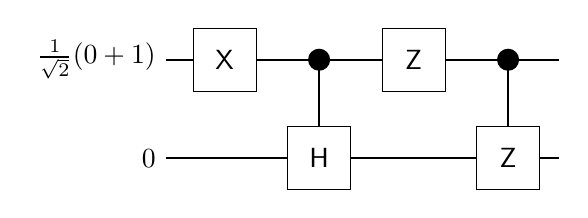
\begin{tikzpicture}[x=1cm,y=1cm]
      \draw[quantum wire] (0,0) -- (5,0);
      \draw[quantum wire] (0,-1.25) -- (5,-1.25);
      \node[anchor=east] at (0,0) {\(\frac{1}{\sqrt{2}}(\ket{0}+\ket{1})\)};
      \node[anchor=east] at (0,-1.25) {\(\ket{0}\)};
      \draw[quantum wire] (1.95,0) -- (1.95,-1.25);
      \draw[quantum wire] (4.35,0) -- (4.35,-1.25);
      \node[quantum gate] at (0.75,0) {X};
      \node[quantum control] at (1.95,0) {};
      \node[quantum gate] at (1.95,-1.25) {H};
      \node[quantum gate] at (3.15,0) {Z};
      \node[quantum control] at (4.35,0) {};
      \node[quantum gate] at (4.35,-1.25) {Z};
    \end{tikzpicture}
  \end{center}
  \begin{enumerate}[label=(\alph*)]
    \item Find the output state.
    \item Is the output state entangled?
    \item What is the probability that a measurement on qubit 2 (after it has gone through the circuit) results in a 0?
  \end{enumerate}
\end{problem}

\begin{problem}{4}
  What does the following circuit do to two arbitrary qubits?
  Use this information to propose a name for this circuit.
  \begin{center}
    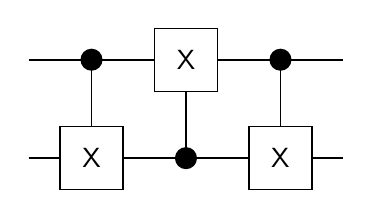
\begin{tikzpicture}[x=1cm,y=1cm]
      \draw[quantum wire] (0,0) -- (4,0);
      \draw[quantum wire] (0,-1.25) -- (4,-1.25);
      \foreach \x in {0.8,2,3.2}
        \draw[quantum wire] (\x,0) -- (\x,-1.25);
      \node[quantum control] at (0.8,0) {};
      \node[quantum gate] at (0.8,-1.25) {X};
      \node[quantum gate] at (2,0) {X};
      \node[quantum control] at (2,-1.25) {};
      \node[quantum control] at (3.2,0) {};
      \node[quantum gate] at (3.2,-1.25) {X};
    \end{tikzpicture}
  \end{center}
\end{problem}
\end{document}
